%!TEX root = ../thesis.tex

\section{実環境の実験}
これまでの節では, いずれもシミュレータ上での実験を行ってきたが, 実験を実環境に移す. それから, 実環境における提案手法の有効性を検証する.

\subsection{実験装置(実環境)}
\begin{itemize}
  \item ロボット
  
  ロボットは前報\cite{okada1}と同様, \figref{Fig:gamma}に示すように, 3つのカメラを搭載したロボットを用いる.

  \vspace{2cm}
  
  \begin{figure}[hbtp]
    \centering
   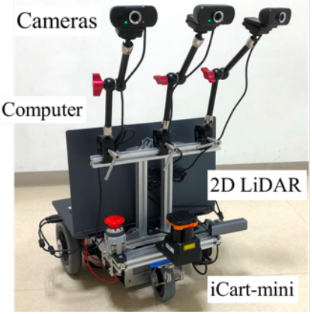
\includegraphics[keepaspectratio, scale=0.7]
        {images/gamma2.png}
   \caption{Experimental setup from \cite{okada1}}
   \label{Fig:gamma}
  \end{figure}

  \newpage

  \item 環境

  \figref{Fig:real_environment}に示すような千葉工業大学津田沼キャンパス2号館3階で実験を行う.

  \begin{figure}[h]
    \centering
    \begin{minipage}[b]{120mm}
      \centering
      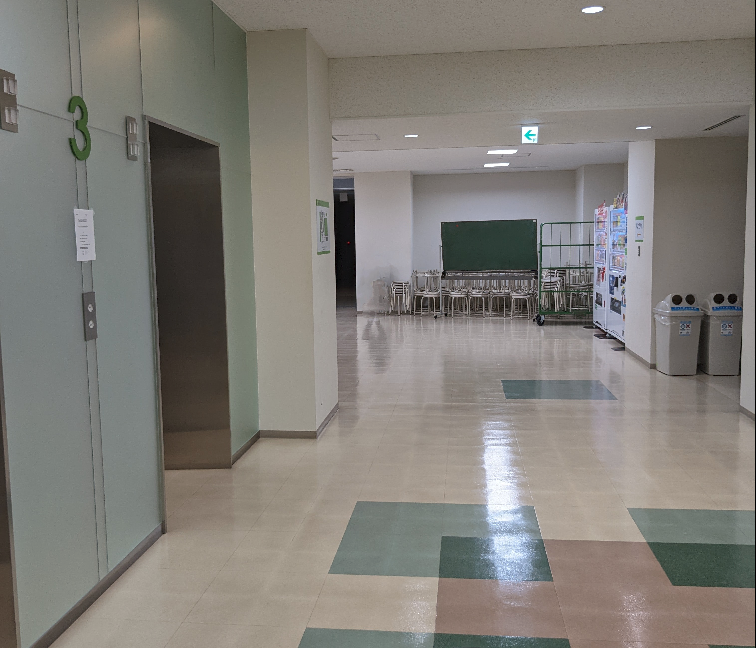
\includegraphics[width=40mm]{images/real.png}
      \caption*{(a) One place in the real environment}
    \end{minipage} 
    % \newpage
    % \hspace{0.03\columnwidth}
    \begin{minipage}[b]{120mm}
      \centering
      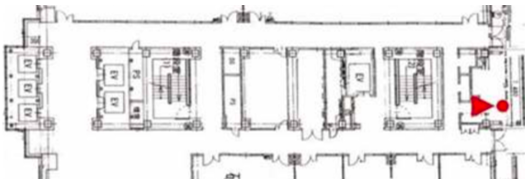
\includegraphics[width=95mm]{images/tsudanuma_structure.png}
      \caption*{(b) structure}
    \end{minipage}
    \caption{Real environment}
    \label{Fig:real_environment}
  \end{figure}
\end{itemize}

\subsection{実験方法}
4.2の実験により, 20000stepほど学習させることで, 十分な成功率が得られる可能性が高いことがわかっている. しかし, 実環境で行う実験時間を削減するため, 実環境に似たシミュレータ上で訓練した学習器をファインチューニングする. なお, 本論文ではファインチューニングによる実験結果の影響を議論しない. 実環境における実験の流れを以下に示す.
\begin{enumerate}
  \item 事前に4.3の実験に倣って, シミュレータ上で10000step学習させる. 
  \item 前段階の学習器を用いて初期値を設定し, 実環境で4.1.2 で示した経路を繰り返し走行させる.
  \item 学習を10000step実行後, テストフェーズに移行する. テストフェーズで正しい順序で経路を選択し, 走行を行えるか確認する.
\end{enumerate}
この一連の流れを 10 回繰り返し行う.

\subsection{実験結果}
実験結果を \figref{Fig:real_result} に示す. この図は, それぞれの走行パターンにおいて正しく経路を選し, 走行できた回数を表している. \tabref{table:real} に実験ごとに全パターンを合計した結果を示す. \tabref{table:real} に示すように, 目標方向に従って 78/120 回, 正しい経路を選択する様子が見られた.
% \par

\begin{figure}[hbtp]
  \centering
 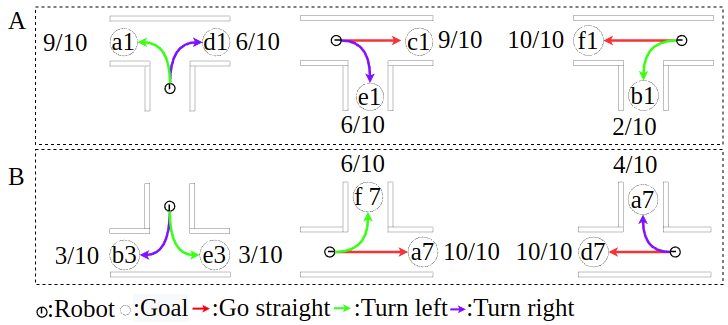
\includegraphics[keepaspectratio, scale=0.5]
      {images/real_result.png}
 \caption{Experimental results for each moving pattern by real environment}
 \label{Fig:real_result}
\end{figure}

\begin{table}[hbtp]
  \caption{Experimental results}
  \label{table:real}
  \centering
  \begin{tabular}{|c|c|c|}
    \hline
    Experiments & Step & Total results\\
    \hline
    Approach1+2 (Simulator similar to real environment) & 20000 & 114/120(95\%)\\
    \hline
    Approach1+2 (Real environment) & 20000 & 78/120(65\%)\\
    \hline
  \end{tabular}
\end{table}

実環境における実験の成功率が著しく低い結果となった. このような結果になった原因について, 考えられるのは以下の3点である.

% \begin{itemize}
%   \item データセットに加えられるカメラ画像に人などが多く写ってしまった
%   \item データセットに加えられるカメラ画像に入る光量が変化してしまった
%   \item カメラ画像の視野角がシミュレータと実環境で違う
% \end{itemize}

\begin{enumerate}
  \item データセットに加えられるカメラ画像に人などが多く写ってしまった
  \item データセットに加えられるカメラ画像に入る光量が変化してしまった
  \item 取得するカメラ画像の視野角と高さがシミュレータと実環境で違う
\end{enumerate}

上記の1,2に関して, シミュレータ上での実験では環境中の光や障害物の有無が変わらない. 一方で, 実環境での実験では通行人の存在や僅かな光の変化がある. 
\par
\figref{Fig:horizonal}はシュミレータ上と実環境で対応する場所で取得した画像を示している. この図より, 視野角と高さが異なっていることがわかる. このことから, 上記の3に関して同一の場所においても視野角の違いなどにより, 取得できる情報量に差が出ている可能性がある.

\begin{figure}[h]
  \centering
  \begin{minipage}[b]{67mm}
    \centering
    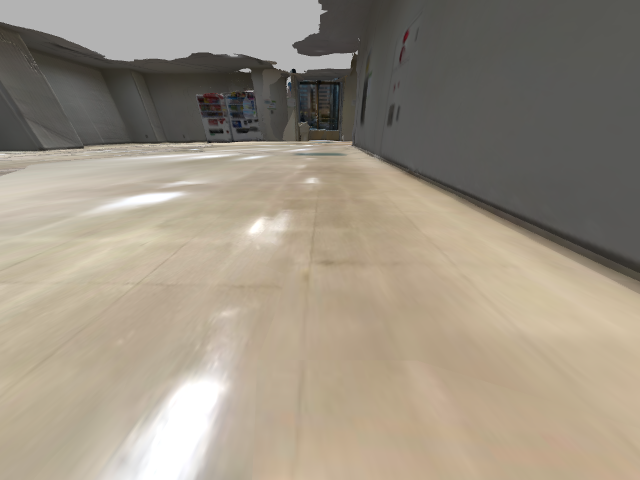
\includegraphics[width=40mm]{images/horizonal_sim.png}
    \caption*{(a) Simulator similar to real environment}
  \end{minipage} 
  % \newpage
  % \hspace{0.03\columnwidth}
  \begin{minipage}[b]{67mm}
    \centering
    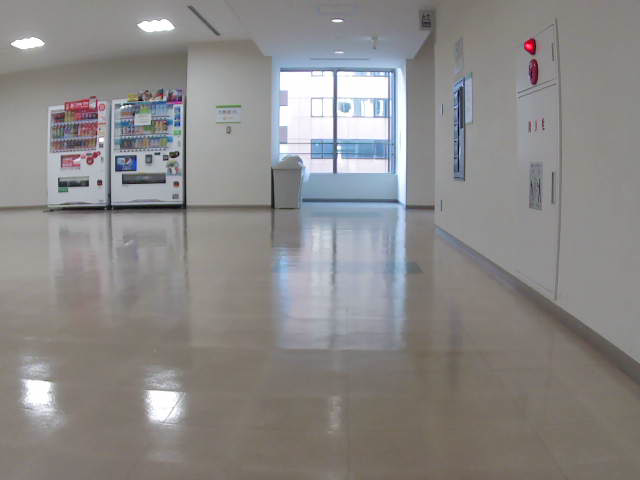
\includegraphics[width=40mm]{images/horizonal_real.png}
    \caption*{(b) Real environment}
  \end{minipage}
  \caption{Acquired camera images at corresponding places}
  \label{Fig:horizonal}
\end{figure}

\figref{Fig:real_model3}は実環境における実験で, 成功率が最多のモデルによる実験結果である. 9/12 回正しい経路を選択する様子が見られた. この図のb3とe3に向かう三叉路などでは, 経路選択前は同じ場所を走行しているため, ほぼ同様の画像が入力されているが, 目標方向に従って正しい経路を選択できている. このことから, 実環境においても提案手法により, 任意の経路選択が行うことができている可能性が高い.
しかし, 成功率が低い原因の解明には未だ至っていない. そのため, 解析は今後の課題となっている.

\begin{figure}[hbtp]
  \centering
 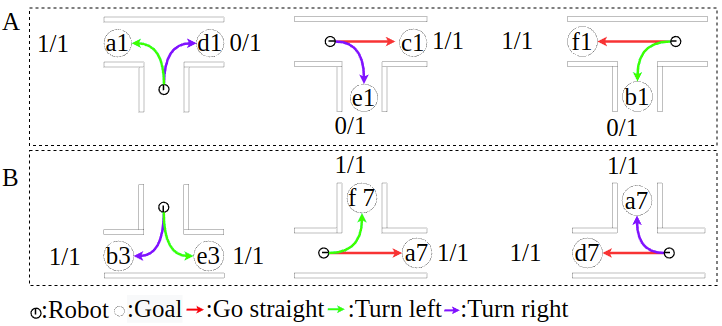
\includegraphics[keepaspectratio, scale=0.45]
      {images/real_model3.png}
 \caption{Experimental results for each moving pattern by models with the highest success rate}
 \label{Fig:real_model3}
\end{figure}

\newpage
